\chapter{Plan}
\label{ch:plan}

\begin{epigraph}
    \textit{I don't let the cleaners in\ldots because \textbf{I} know where
        everything in this room is.  All the books, the papers --- and the moment
        they start cleaning, those things get hopelessly organized and tucked away
        and I can never find them again.} --- Crown of Midnight (2013), Sarah J. Maas
\end{epigraph}

This section lays out my plan for completing the work necessary to explore my
thesis.  In \autoref{ch:plan:sec:existing-work} I summarize work I
have done prior to this thesis proposal.  In \autoref{ch:plan:sec:proposed-work}
I summarize work I expect is required to evaluate my thesis,
consistent with the model that I have laid out in \autoref{ch:architecture}.

\begin{table}[!htb]
    \caption{Summary of Existing Work}
    \label{table:existing-work}
    {\renewcommand{\arraystretch}{1.3} %<- modify value to suit your needs
        \begin{tabular}{p{2cm}p{9cm}}
            Time          & Description                                                        \\
            December 2016 & Original PhD application: ``In my own work I routinely
            find that location information is a challenge because I do not know
            \emph{where} I stored that information.''                                          \\
            May 2017      & CS-50 Celebration Poster Session.
            \autoref{figure:percipience-poster}                                                \\
            January 2019  & Not Dead Yet (HotOS).  Rejected paper submission
            discussed file relationships and suggested graph oriented name spaces
            rather than hierarchical ones.
            \\
            March 2019    & Percipience: Associative File Systems for Unstructured Data
            Relationships (Eurosys Doctoral Workshop). Presented this initial
            description of both my Finesse work (FUSE file systems with a kernel
            bypass) and the Graph file system proposed in the HotOS submission. This
            included a poster (see \autoref{figure:eurosysdw-poster}).
            \\
            January 2021  & Silos are for Grain, not Namespaces (HotOS).  Rejected
            paper submission discussed challenges involved in having distinct
            ``storage silos'' and proposing a potential architecture to solve that
            problem.  Proposed architecture is shown in \autoref{figure:hotos21-nirvana-arch}. \\

            April 2021    & Position: Naming is Hard (HotStorage).  Rejected paper
            submission proposed a rich meta-data focused file location system.
            I used the architecture proposal in the Hot Storage paper as the basis of the
            my architecture in this document (see \autoref{fig:arch}).
        \end{tabular}
    }%
\end{table}

\section{Existing Work}
\label{ch:plan:sec:existing-work}

This basic question about \emph{finding} is rooted in work that I have done
throughout my time at UBC.  I have summarized that work in
\autoref{table:existing-work}.

A key take-away from the feedback I have received over the years is that being
able to demonstrate a working system is an important part of convincing the
community to accept this work.  This has influenced my proposal --- it adopts
many of the ideas that I have proposed and focuses on demonstrating them in a
tangible, measurable fashion to provide the level of contribution required for
them to be useful to the systems research community.

\begin{figure}[!htb]
    \centering
    \caption{Percipience: Finding Your Personal Data \\Presented at UBC CS-50 Poster Session}
    \label{figure:percipience-poster}
    \includegraphics[width=0.95\textwidth]{figures/sapience-poster.pdf}
\end{figure}

\begin{figure}[!htb]
    \centering
    \caption{Percipience: Finding the \emph{Right} Data \\ Presented at Eurosys
        Doctoral Workshop}
    \label{figure:eurosysdw-poster}
    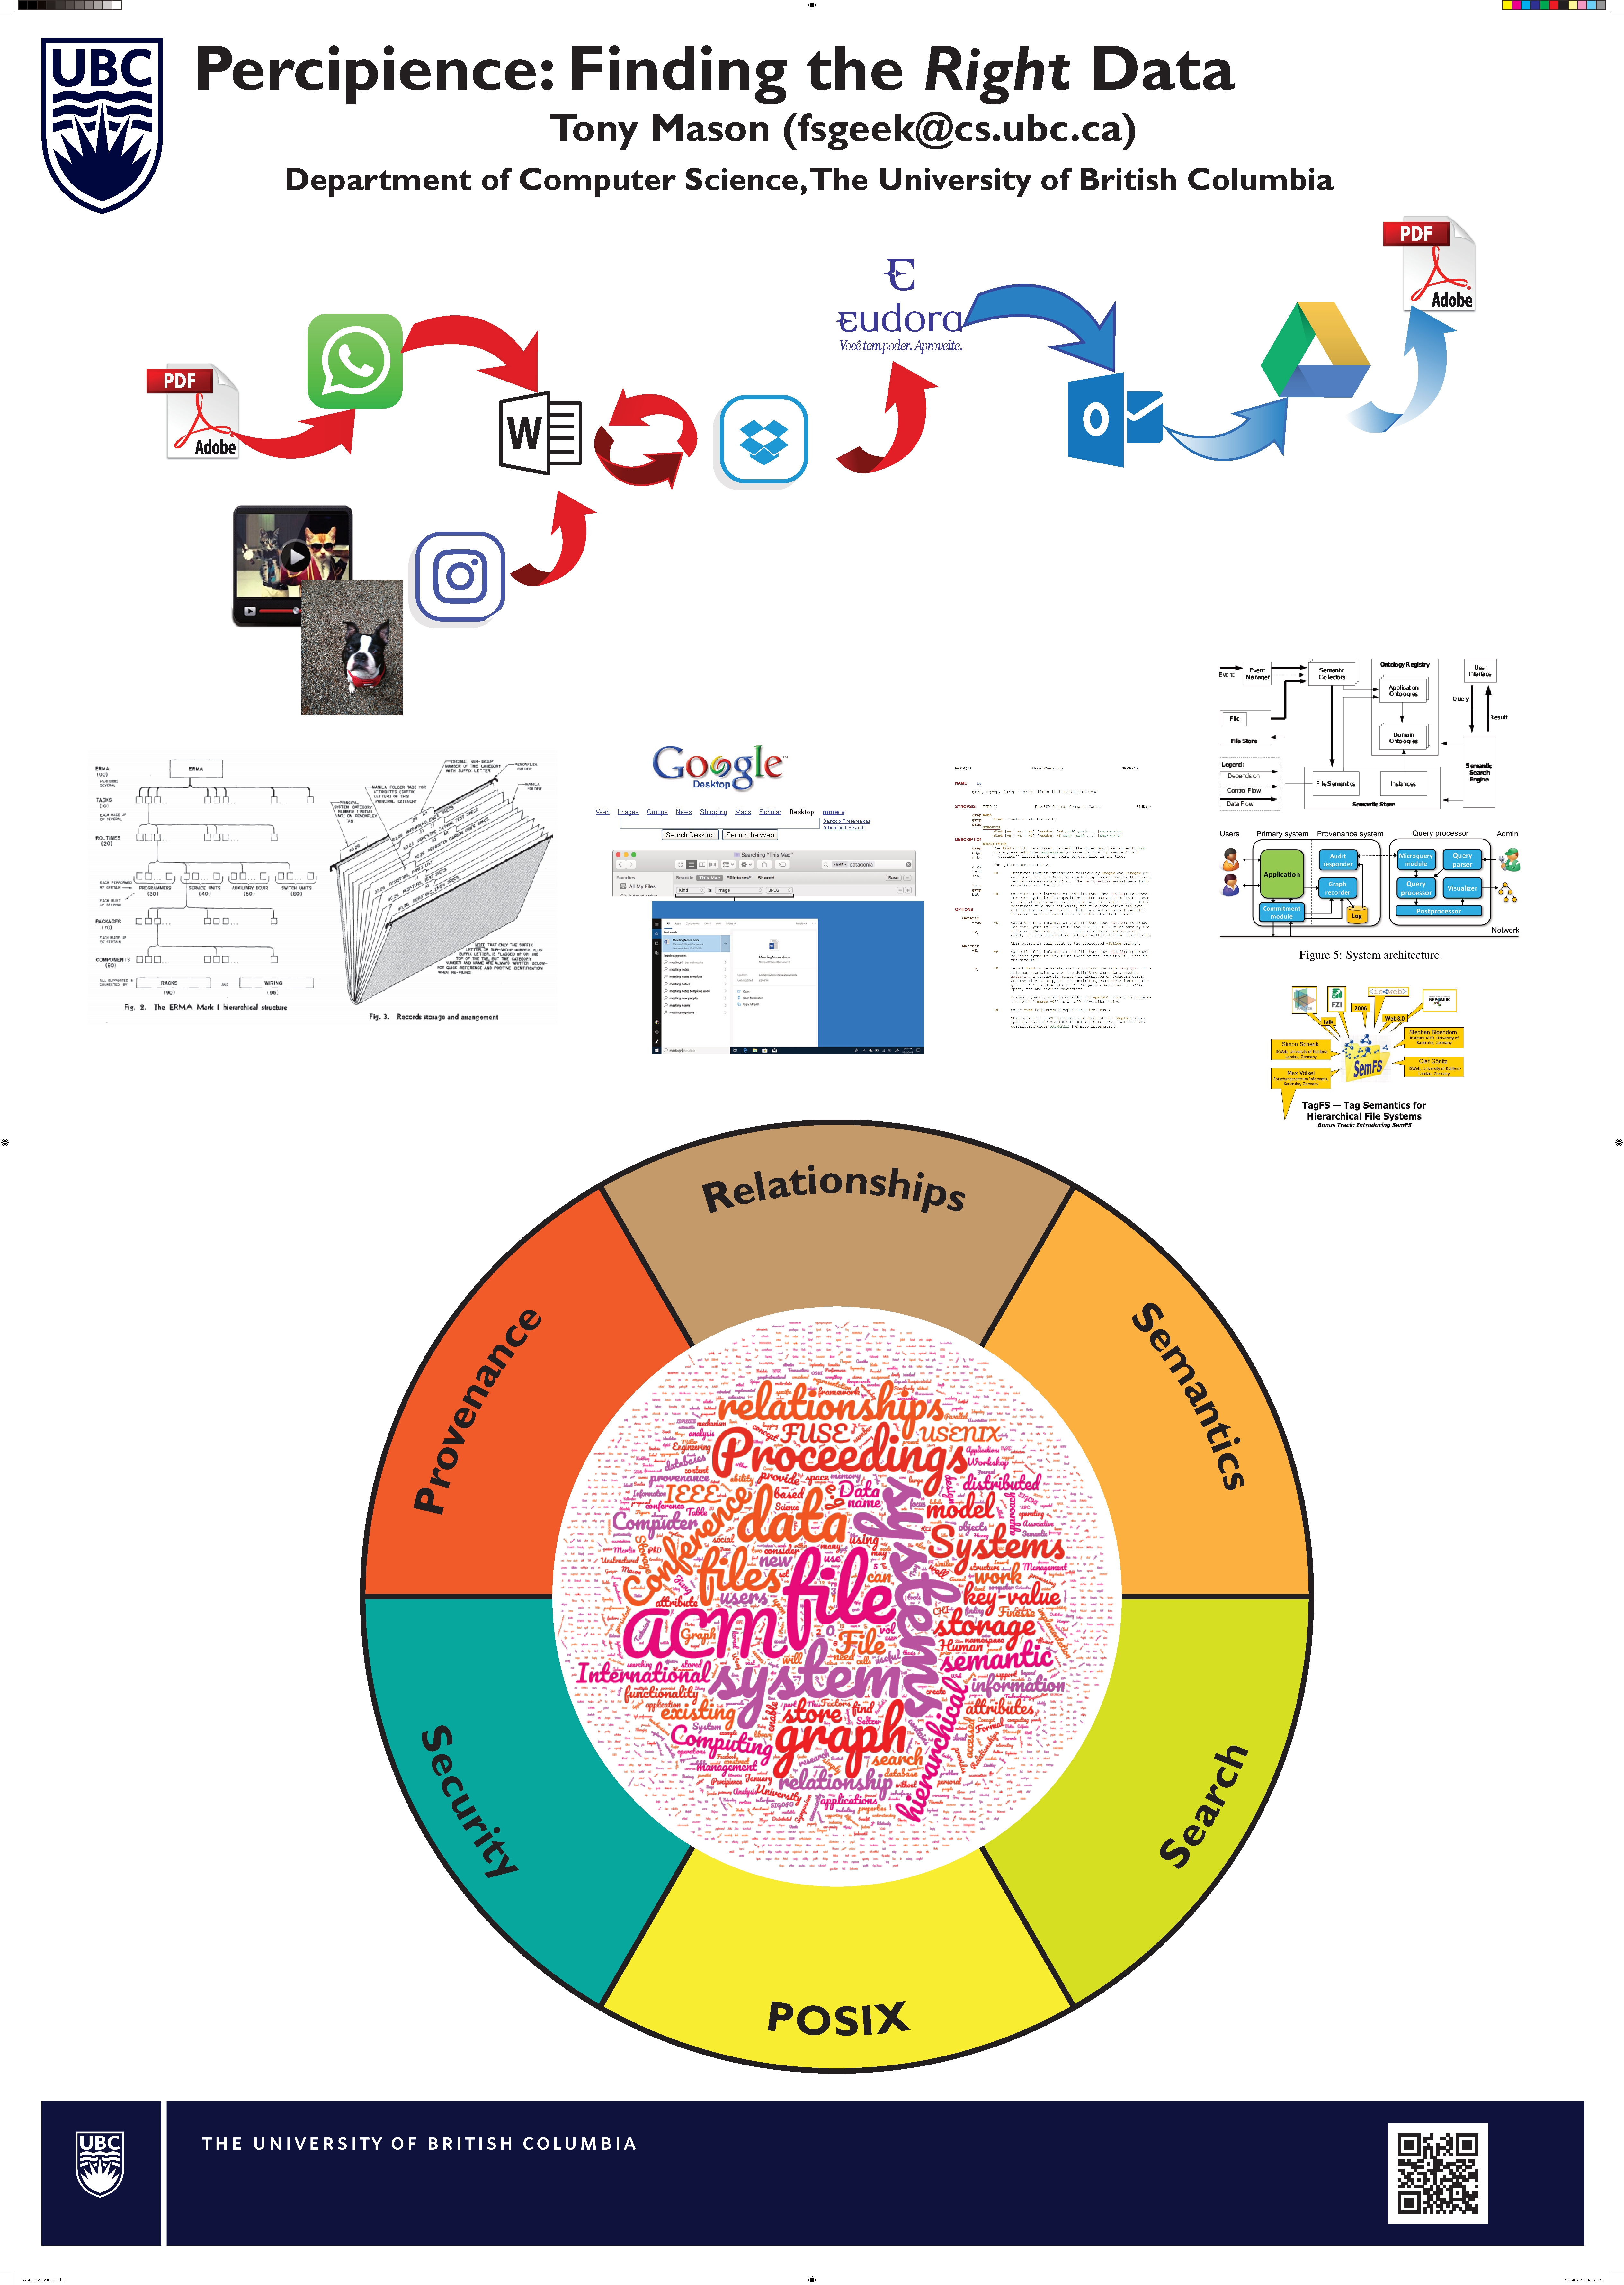
\includegraphics[width=0.95\textwidth]{figures/eurossys-dw-poster.pdf}
\end{figure}

\begin{figure}[!htb]
    \centering
    \caption{Nirvana Systems Architecture \\ Included in Rejected HotOS 2021 submission}
    \label{figure:hotos21-nirvana-arch}
    \includegraphics[width=0.95\textwidth]{reference/hotos21/figures/nirvana-arch-8.png}
\end{figure}


\section{Proposed Work}
\label{ch:plan:sec:proposed-work}

My plan is to utilize existing tools to build a dataset on a single
node system using data that can be easily obtained.  That will assist me in
ensuring I can address research questions \ref{rq:define-ac} and
\ref{rq:rich-data}.  My goal is to ensure that I collect and convert that
information into a usable data format (research question \ref{rq:capture-ac}.)
With an actual data set, I can use it to perform additional analysis, create
exploratory prototypes and share data sets with others when possible.

While existing evidence suggests that \emph{activity context} will improve
``associative access to files,'' which I interpret to mean
that it improves the ability to find relevant content I need to construct enough
of the system I have proposed in \autoref{ch:architecture} to confirm that I can
reproduce those results.  Thus, my focus will be on utilizing existing
data sources in modern operating systems for extracting activity information,
which can be easily converted into the events needed for the activity context.
The benefit of this approach is it minimizes development risk while building the
infrastructure needed to extend the activities that are collected.

Once that is done, my plan is to move towards answering research question
\ref{rq:meta-data-query}, which will require that I evaluate existing models
suitable for querying across the meta-data that represents activity context and
either pick one or derive a model that is suitable for my use.  Once that is
done, I can work with collaborators to use this interface with existing and/or
potential new tools.

Finally, with the activity context collection and query infrastructure, I will
turn my attention towards identifying at least one novel new type of activity
context, ideally in collaboration with others who are evaluating ways to extend
\emph{finding} tools they have built against my interface and adding that to the
system.  This will allow me to evaluate the ease (or difficulty) of extending
the activity context system as well as the additional effort required to enable
tools to take advantage of that new functionality.

Thus, I envision my work in supporting my thesis to logically consist of three
stages:

\begin{enumerate}
    \item \label{plan:basic-system-construction}\textbf{Basic System Construction}.  In this stage I will look at
          existing components that can be used to build some or all of the
          architecture described in \autoref{ch:architecture} within some constrained
          environment, such as the digital content and the activity context generated
          by the devices of a single user.  I review my anticipated work for
          this portion of the project in \autoref{plan:basic-system}

    \item \label{plan:acql}\textbf{Activity Context Query Language}.  In this stage I will review
          potential interfaces for querying activity contexts, adopt one or adapt one
          or more systems and then implement and evaluate that.  This is likely to
          involve iteration between the system, tools, and query language to find a
          viable balance between the three. It is premature to project this
          anticipated work, though I do provide a rough time estimate in
          \autoref{plan:schedule}.

    \item \label{plan:new-activity}\textbf{Novel activity context}.  In this
          stage I will work to identify at least one novel type of activity context
          information that is not presently available on at least one system.  That
          new activity context will then be used to design a new activity context
          event provider that integrates with the basic system (stage
          \ref{plan:basic-system-construction}) and query language (state
          \ref{plan:acql}) to support the new activity context event.  It is likely
          that there will be yet another feedback cycle between these components in
          order to simplify the extensibility and usability of new activity context
          events. It is premature to project this anticipated work, though I do
          provide a rough time estimate in \autoref{plan:schedule}.

\end{enumerate}

Given the generality of this plan, there should be sufficient flexibility to
adapt to the actual findings from my activities in supporting this research as
well as any collaborations that might arise during the course of completing my
thesis work.

\section{Basic System}
\label{plan:basic-system}

My intial plan is to utilize existing system components for gathering activity
context.  For example, the extended Berkeley Packet Filter (eBPF) is an
extensive data collection mechanism available on both Linux and Windows systems.
It provides a mechanism for adding data gathering elements to an existing
operating system in a way that is commensurate with my understanding of
\emph{activity context}.

This information will then be stored within the system that I have proposed in
\autoref{ch:architecture}.  To review, the services that will be implemented in this phase of my work are:

\begin{description}
    \item[Metadata Servers] --- there are existing models for meta-data servers,
        such as Egeria~\footnote{\url{https://github.com/odpi/egeria}} or
        Amundsen~\footnote{\url{https://github.com/amundsen-io/amundsen}} (a
        demonstrative, but not definitive list) that might be sufficient. If
        not, using a key-value store such as
        WiredTiger~\footnote{\url{https://github.com/wiredtiger/wiredtiger}} to
        construct a metadata server is also viable. It may also be possible to
        simply use an appropriate cloud hosted solution.  My goal here is to use
        an existing solution, not build something new.

    \item[Namespace Servers] --- my expectation is that this will need to be
        constructed; it must interoperate with the metadata servers.  Work here will
        include defining the interface to constructing a new namespace or retrieving
        a previously constructed namespace. While the ultimate goal is to have a
        federated namespace service, this initial effort need only provide a single,
        non-federated namespace even though that is more limited than the actual
        design.

    \item[Activity Monitors] --- these create the activity context information I
        described previously.  I would expect that only a single activity monitor
        will be built for this initial system prototype and the details of this will
        be driven by the chosen definition of the activity context and relevant
        activity providers.

    \item[Attribute Services] --- because \system is a naming system, we need a
        mechanism that retrieves storage attributes. Initially, this will consist of
        a source for scanning current content and then a monitoring mechanism
        (likely similar to the activity provider) that notifies the attribute
        service to update the attributes of files that have changed.

    \item[Update Notification Server] --- existing systems provide change
        notifications.  In a cross-silo system this sort of dynamic state monitoring
        will also be useful.  An initial implementation for a local system could
        consist simply of using the existing change notification mechanism(s) for
        watching changes.  A more robust implementation could use information from
        the meta-data service(s) to determine if a given change is of interest.
        This dynamic change tracking could then be federated as part of the later
        planned work.
\end{description}

For initial analysis, I propose using the existing storage silos that I
identified in \autoref{ch:background:sec:storage-silos} and combining
information about access to them on the local device with the other information
that I have identified plus additional information I expect to identify in
collaboration with others to form the raw data that is used by the
\emph{activity context}.

\section{Schedule}
\label{plan:schedule}

% Table generated by Excel2LaTeX from sheet 'Sheet1'
\begin{table}[htbp]
  \centering
  \caption{Proposed Schedule for competion of Doctoral Thesis}
  \begin{tabular}{p{0.15\columnwidth}p{0.85\columnwidth}}
    \textbf{Month} & \textbf{Activity}                                          \\
    \rowcolor[HTML]{C0C0C0} \multicolumn{2}{c}{2021}                            \\
    September      & Draft thesis proposal to supervisors                       \\
    October        & Updated draft thesis proposal to supervisors               \\
    November       & Final thesis proposal to committee                         \\
    December       & Defend thesis proposal - reach candidacy                   \\
    \rowcolor[HTML]{C0C0C0} \multicolumn{2}{c}{2022}                            \\
    January        & Begin proposed research Part 1 (Storage Silo)              \\
    April          & Milestone 1 Storage Silo (Alpha)                           \\
    June           & Milestone 2: Storage Silo (Beta)                           \\
    August         & Milestone 3: Storage Silo (Complete)                       \\
    September      & Storage Silo paper submission ready                        \\
    September      & Begin proposed research Part 2 (Federated Naming/Security) \\
    December       & Milestone 1: Federated Naming/Security (Alpha)             \\
    \rowcolor[HTML]{C0C0C0} \multicolumn{2}{c}{2023}                            \\
    March          & Milestone 2: Federated Naming/Security (Beta)              \\
    June           & Milestone 3: Federated Naming/Security (Complete)          \\
    July           & Federated Naming/Security Paper submission ready.          \\
    September      & Milestone 1: Cross-Silo Naming (Alpha)                     \\
    December       & Milestone 2: Cross-Silo Naming (Beta)                      \\
    \rowcolor[HTML]{C0C0C0} \multicolumn{2}{c}{2024}                            \\
    March          & Milestone 3: Cross-Silo Naming (Complete)                  \\
    April          & Cross-silo Naming Paper submission ready                   \\
    June           & Draft thesis.                                              \\
    August         & Final thesis.                                              \\
    October        & Defend thesis.                                             \\
  \end{tabular}%
  \label{ch:plan:tab:schedule}%
\end{table}%


In \autoref{table:schedule} I have proposed a \emph{pro forma} plan for
completing the work required for my thesis.  It is subject to revision as I
gather additional data, answer research questions, and iterate over data
collection processes.  If I am able to find collaborators, their feedback will
be invaluable but I have worked to ensure I can make forward progress towards
completing my thesis work alone.

In the schedule I use the following terms:

\begin{description}
    \item[Alpha] - I define an ``alpha release'' as being a functional but
        feature restricted version of the proposed project.  This may mean there are
        known issues and limitations with the tools that I have built.  Such a
        milestone would ordinarily provide useful insight into general direction and
        yield some useful information for consideration.

    \item[Beta] - I define a ``beta release'' as being a functional version of
        the proposed project deliverables (e.g., working tools).  There can still be
        outstanding issues to address but it should be functionally complete.  At
        this stage details such as data formats would not normally change. Such a
        milestone should provide substantial insight into the shape of the final
        project deliverables.

    \item[Complete] - I define a ``complete release'' as being a functional
        version of the project tools and the outline of my findings draft form.
        Findings will ordinarily be delivered in the format of a publication focused
        write-up of findings and a separate document describing the tools that I
        have constructed, how the data was generated, and the location of
        information that I collected as the basis of my write-up.

    \item[Write-Up] The project write-up will consist of a submission-ready
        paper format, in addition to any revisions necessary to tool documentation
        and updated or additional data sets.

\end{description}

I have not attempted to align these milestones to specific conference submission
deadlines as it seems to be premature to consider appropriate venues for
submitting specific works.

\textbf{Note:} there is a realistic likelihood that this project will not
achieve a uniform rate of publication submission and/or acceptance.  While I
have tried to ``front load'' some of the work in order to permit publication of
results early, a common feedback in prior submissions has been that reviewers
want to see something real to evaluate.  Thus, I am providing a description of
the deadlines for venues that I see as relevant to submission of my work.  Dates
for conferences after 2022 are speculative and subject to change.

\begin{table}
    \centering
    \caption{Potential Conferences for Submission 2022-2024}
    \label{table:conferences}
    {\renewcommand{\arraystretch}{1.3} %<- modify value to suit your needs
        \begin{tabular}{p{4cm}p{4cm}p{4cm}ccl}
            \multicolumn{2}{c}{Dates} & Venue Name                       \\
            Conference                & Submission                       \\
            \\
            \rowcolor[rgb]{ .751,  .751,  .751} \multicolumn{3}{c}{2022} \\
            June 13-15                & March 1           & ACM SYSTOR   \\
            July 11-13                & December 14, 2021 & USENIX OSDI  \\
            July 11-13                & January 13        & USENIX ATC   \\
            September 5-9             & March 1           & VLDB         \\
            \\
            \rowcolor[rgb]{ .751,  .751,  .751} \multicolumn{3}{c}{2023} \\
            February                  & September 2022    & USENIX FAST  \\
            April                     & October 2022      & ACM Eurosys  \\
            June                      & March             & ACM SYSTOR   \\
            June                      & March             & SIGMOD       \\
            July                      & December 2022     & USENIX OSDI  \\
            July                      & January           & USENIX ATC   \\
            September                 & March             & VLDB         \\
            October                   & April             & ACM SOSP     \\
            \\
            \rowcolor[rgb]{ .751,  .751,  .751}\multicolumn{3}{c}{2024}  \\
            February                  & September 2023    & USENIX FAST  \\
            April                     & October 2023      & ACM Eurosys  \\
            June                      & March             & ACM SYSTOR   \\
            June                      & March             & SIGMOD       \\
            July                      & December 2022     & USENIX OSDI  \\
            July                      & January           & USENIX ATC   \\
            September                 & March             & VLDB         \\
        \end{tabular}
    }
\end{table}

In \autoref{table:conferences} I have listed potential conferences that seem
relevant to my proposed research; the actual venue chosen for submission is
subject to change but should be of comparable quality to those I have suggested.
